\documentclass[aspectratio=169]{beamer}

\usepackage[round,authoryear]{natbib}
\usepackage{tikz}
\usepackage{standalone}
\usepackage{adjustbox}

\setbeamertemplate{navigation symbols}{}
\setbeamertemplate{headline}{}
\setbeamertemplate{footline}[frame number]
\setbeamertemplate{itemize item}[circle]
\setbeamertemplate{itemize subitem}[circle]
\setbeamertemplate{itemize subsubitem}[circle]

% Display alert blocks inline, using the title color and surrounding text size.
\renewenvironment{alertblock}[1]{%
    \par\medskip\noindent
    {\usebeamercolor[fg]{frametitle}#1}\enspace
    \ignorespaces
}{%
    \par\medskip
}

\title{Moral Hazard versus Liquidity in Household
Bankruptcy}
\subtitle{Indarte (2023)}
\author{Siddhartha Lewis-Hayre}
\date{\today}

\begin{document}

\begin{frame}
    \titlepage
\end{frame}

\begin{frame}{Motivation}

Why do people default?

\vspace{0.3cm}

\begin{itemize}
    \item Popular understanding: because you cannot pay
    \item But default subtle in general equilibrium
    \begin{itemize}
        \item assuming complete markets and cost of default, default is inefficient
    \end{itemize}
\end{itemize}

\vspace{0.3cm}

\centering
\begin{tabular}{l p{0.30\textwidth} p{0.30\textwidth}}
    \hline
    & \textbf{Moral Hazard} & \textbf{Liquidity} \\
    \hline
    Effect & Transfer & Consumption smoothing \\
    Literature & Geanakoplos (2010) & Chatterjee et al. (2007) \\
    Amplification & Leverage cycle & Procyclical credit \\
    Policy & Debt forgiveness & Liquidity injection\\
    \hline
\end{tabular}
\end{frame}

\begin{frame}{Motivation}
    \begin{alertblock}{Question:}
        Why do households declare bankruptcy?
    \end{alertblock}

    \vspace{0.3cm}

    \begin{alertblock}{Goal:}
        Identify causal impact of the moral hazard and liquidity effects on filing
    \end{alertblock}

    \vspace{0.3cm}

    Causal estimate would quantify the trade-off between moral hazard and consumption smoothing

\end{frame}

\begin{frame}{Challenges}
    How to identify causal impact of the moral hazard and liquidity effects on filing?
    \vspace{0.3cm}

    \textbf{Moral Hazard:}
    \begin{itemize}
        \item cross sectional variation has ommited variables that lower wealth and increase filing
        \begin{itemize}
            \item[$\rightarrow$] overestimates effect
        \end{itemize}
        \item policy variation combines direct effect and GE effect of lending contraction
        \begin{itemize}
            \item[$\rightarrow$] underestimates effect
        \end{itemize}
    \end{itemize}
    \vspace{0.3cm}
    \textbf{Liquidity}
    \begin{itemize}
        \item find liquidity shock that is not seizable in bankruptcy
        \item otherwise liquidity shock will decrease moral hazard
        \begin{itemize}
            \item[$\rightarrow$] if liquidity shock is seizable, overestimates liquidity effect
        \end{itemize}
    \end{itemize}
\end{frame}

\begin{frame}{Methodology}

\textbf{Moral Hazard:}
\begin{itemize}
    \item exploits homestead exemption laws
    \item regression kink design (RKD) around equity distance from exemption
    \item \textit{Identification assumption:} other factors affecting filing are smooth at kink
\end{itemize}
\vspace{0.3cm}
\textbf{Liquidity}
\begin{itemize}
    \item liquidity shock from reset rates of ARM
    \item instruments reset payment with ARM indexation to Libor versus Treasuries
    \item \textit{Identification assumption:} ARM indexation rate only affects filing through mortgage payment
\end{itemize}
    
\end{frame}

\begin{frame}{Summary of Results}

\textbf{Moral Hazard:}
\begin{itemize}
    \item \$1K decrease in generosity of bankruptcy reduces filing rate by \textbf{0.02pp}
\end{itemize}
\textbf{Liquidity:}
\begin{itemize}
        \item \$1K decrease in annual mortgage payment reduces filing rate by \textbf{0.09pp}
    \end{itemize}

\vspace{0.3cm}

\begin{itemize}
    \item[{\usebeamercolor[fg]{itemize item}$\Rightarrow$}] \textbf{Liquidity effect five} times larger than moral hazard effect
\end{itemize}

\vspace{0.3cm}

If you decrease dischargeable debt, \textbf{83\%} of filing response is due to \textbf{liquidity}

% \begingroup
% \setbeamercolor{frametitle}{fg=red}
% \begin{alertblock}{Critique:}
%     From a policy perspective, if you do not know who is going to file, it would be much cheaper to increase bankruptcy generosity than to give handouts to everyone
% \end{alertblock}
% \endgroup

\end{frame}

\begin{frame}[plain]
    \centering
    {\usebeamercolor[fg]{frametitle}\Huge\bfseries Moral Hazard Effect}
\end{frame}

\begin{frame}{Homestead Exemption}
    \centering
    \begin{adjustbox}{width=0.8\textwidth,max totalheight=0.8\textheight,center}
        \input{images/homestead_exemption.tex}
    \end{adjustbox}
\end{frame}

\begin{frame}{Stilized Bankruptcy Balance Sheet}
    \vspace{0.2cm}
    \centering
    \begin{adjustbox}{width=\textwidth,max totalheight=\textheight,center}
        % Include with \input{bankruptcy_balance_sheet.tex}.
% Requires \usepackage{tikz}.
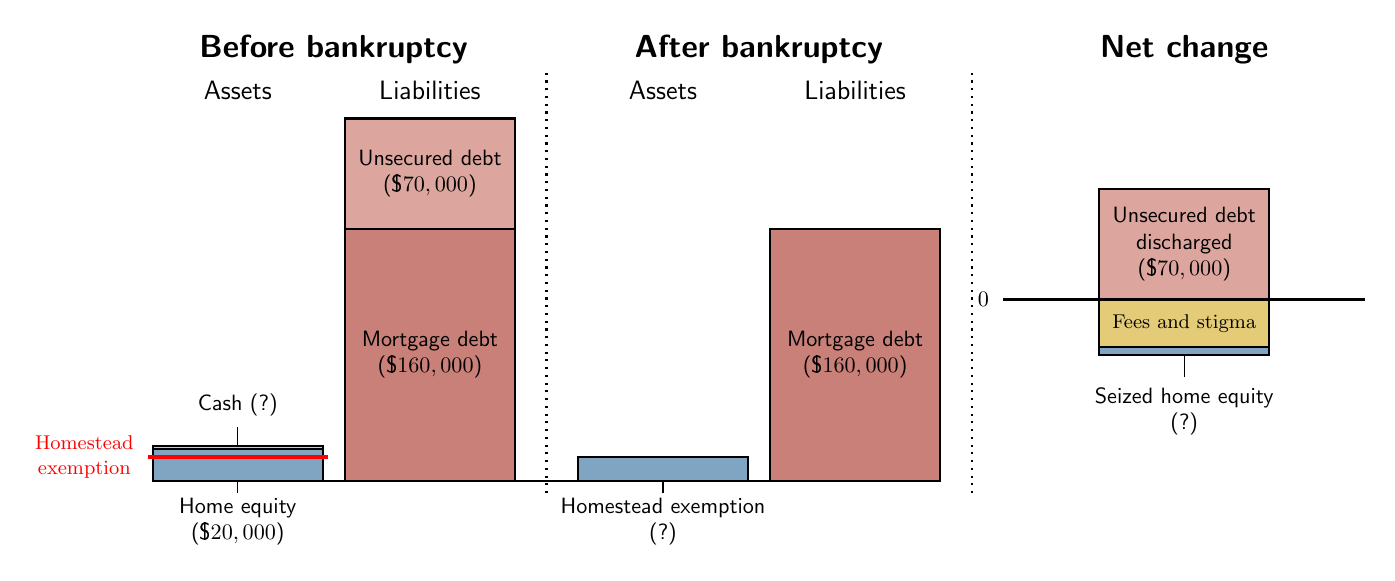
\begin{tikzpicture}[
    font=\sffamily,
    scale=0.8,
    every node/.style={transform shape}
]

% Muted fill colors (editable).
\definecolor{cashfill}{HTML}{E3CB78}
\definecolor{debtfill}{HTML}{C98078}
\definecolor{unsecuredfill}{HTML}{DCA69E}
\definecolor{equityfill}{HTML}{7FA5C2}

% =========================
% Editable amounts (thousands of dollars).
% 2025 BAPCPA Table 1D: national totals / 181,587 complete schedules.
% Mortgage debt proxies all secured claims; home equity proxies real property
% minus secured claims. Unsecured debt uses nonpriority unsecured claims.
% https://www.uscourts.gov/sites/default/files/document/bapcpa_1d_1231.2025.pdf
% Cash: 3 * (2021 ABI monthly income 3,513 - monthly expenses 2,810).
% https://abi-org.s3.amazonaws.com/Covid19/stats/Weekly_Update_Dec_6-12_2021.pdf
% This stylized illustration mixes years; exempt equity is assumed to be 75%.
% Displayed dollar amounts and their box sizes are rounded to the nearest $10,000.
% =========================
\def\cash{2.109}
\def\homeequity{20}
\def\mortgagedebt{160}
\def\unsecureddebt{70}
\def\legalfees{2}
% Illustrative height for legal fees and stigma, including nonmonetary costs.
\def\legalcostheight{0.75}
\pgfmathsetmacro{\exemptassets}{0.75*\homeequity}
\newcommand{\amountlabel}[1]{(\$\pgfmathprintnumber[fixed,precision=0,1000 sep={,}]{#1e3})}

% Geometry: common height-per-unit scale before and after bankruptcy.
\def\heightperunit{0.025}
\def\barwidth{2.7}
\def\columngap{0.35}
\def\panelgap{1.0}
\pgfmathsetmacro{\debt}{\mortgagedebt+\unsecureddebt}
\pgfmathsetmacro{\top}{\heightperunit*max(\cash+\homeequity,\debt,\exemptassets)}
\pgfmathsetmacro{\panelwidth}{2*\barwidth+\columngap}
\pgfmathsetmacro{\panelshift}{\panelwidth+\panelgap}
\pgfmathsetmacro{\debtx}{\barwidth+\columngap}
\pgfmathsetmacro{\lostequity}{\homeequity-\exemptassets}
\pgfmathsetmacro{\netpanelshift}{2*\panelshift}
\pgfmathsetmacro{\netbaseline}{\top/2}

% =========================
% Left: Before bankruptcy
% =========================
\node at ({\panelwidth/2},{\top+1.1}) {\Large\textbf{Before bankruptcy}};
\node at ({\barwidth/2},{\top+0.45}) {\large Assets};
\node at ({\debtx+\barwidth/2},{\top+0.45}) {\large Liabilities};

% Assets: home equity below cash.
\draw[thick,fill=equityfill] (0,0) rectangle (\barwidth,{\heightperunit*\homeequity});
\node[align=center] at ({\barwidth/2},-0.65) {Home equity\\\amountlabel{\homeequity}};
\draw[thin] ({\barwidth/2},-0.2) -- ({\barwidth/2},0);
% Assumed exemption threshold: 75% of initial home equity.
\draw[red,very thick] (-0.08,{\heightperunit*\exemptassets})
    -- ({\barwidth+0.08},{\heightperunit*\exemptassets});
\node[red,align=center,anchor=east,font=\small]
    at (-0.18,{\heightperunit*\exemptassets}) {Homestead\\exemption};
\draw[thick,fill=cashfill] (0,{\heightperunit*\homeequity})
    rectangle (\barwidth,{\heightperunit*(\homeequity+\cash)});
% Place the cash label outside its proportionally small box.
\node[align=center,anchor=south] at ({\barwidth/2},{\heightperunit*(\homeequity+\cash)+0.35}) {Cash (?)};
\draw[thin] ({\barwidth/2},{\heightperunit*(\homeequity+\cash)})
    -- ({\barwidth/2},{\heightperunit*(\homeequity+\cash)+0.3});

% Liabilities: mortgage debt below unsecured debt.
\draw[thick,fill=debtfill] (\debtx,0)
    rectangle ({\debtx+\barwidth},{\heightperunit*\mortgagedebt});
\node[align=center] at ({\debtx+\barwidth/2},{\heightperunit*\mortgagedebt/2}) {Mortgage debt\\\amountlabel{\mortgagedebt}};
\draw[thick,fill=unsecuredfill] (\debtx,{\heightperunit*\mortgagedebt})
    rectangle ({\debtx+\barwidth},{\heightperunit*\debt});
\node[align=center] at ({\debtx+\barwidth/2},{\heightperunit*(\mortgagedebt+\unsecureddebt/2)}) {Unsecured debt\\\amountlabel{\unsecureddebt}};

\draw[dotted,thick]
    ({\panelwidth+\panelgap/2},-0.2) --
    ({\panelwidth+\panelgap/2},{\top+0.8});

% =========================
% Right: After bankruptcy
% =========================
\begin{scope}[xshift={\panelshift cm}]
    \node at ({\panelwidth/2},{\top+1.1}) {\Large\textbf{After bankruptcy}};
    \node at ({\barwidth/2},{\top+0.45}) {\large Assets};
    \node at ({\debtx+\barwidth/2},{\top+0.45}) {\large Liabilities};

    \draw[thick,fill=equityfill] (0,0) rectangle (\barwidth,{\heightperunit*\exemptassets});
    \node[align=center] at ({\barwidth/2},-0.65) {Homestead exemption\\(?)};
    \draw[thin] ({\barwidth/2},-0.2) -- ({\barwidth/2},0);

    % Mortgage debt remains; unsecured debt is discharged.
    \draw[thick,fill=debtfill] (\debtx,0)
        rectangle ({\debtx+\barwidth},{\heightperunit*\mortgagedebt});
    \node[align=center] at ({\debtx+\barwidth/2},{\heightperunit*\mortgagedebt/2}) {Mortgage debt\\\amountlabel{\mortgagedebt}};

\end{scope}

% Common baseline across both panels.
\draw[thick] (0,0) -- ({2*\panelwidth+\panelgap},0);

% =========================
% Third panel: gains and losses relative to a central zero line.
% Positive values are debt relief; negative values are legal fees and lost home equity.
% Use the same height-per-dollar scale as the first two panels.
% =========================
\draw[dotted,thick]
    ({2*\panelwidth+1.5*\panelgap},-0.2) --
    ({2*\panelwidth+1.5*\panelgap},{\top+0.8});
\begin{scope}[xshift={\netpanelshift cm}]
    \node at ({\panelwidth/2},{\top+1.1}) {\Large\textbf{Net change}};
    \pgfmathsetmacro{\netbarleft}{(\panelwidth-\barwidth)/2}
    \pgfmathsetmacro{\netbarright}{(\panelwidth+\barwidth)/2}
    \draw[thick,fill=unsecuredfill]
        (\netbarleft,\netbaseline)
        rectangle (\netbarright,{\netbaseline+\heightperunit*\unsecureddebt});
    \node[align=center] at
        ({\panelwidth/2},{\netbaseline+\heightperunit*\unsecureddebt/2})
        {Unsecured debt\\discharged\\\amountlabel{\unsecureddebt}};
    \draw[thick,fill=cashfill]
        (\netbarleft,\netbaseline)
        rectangle (\netbarright,{\netbaseline-\legalcostheight});
    \node[align=center,font=\small] at
        ({\panelwidth/2},{\netbaseline-\legalcostheight/2})
        {Fees and stigma};
    \draw[thick,fill=equityfill]
        (\netbarleft,{\netbaseline-\legalcostheight})
        rectangle (\netbarright,{\netbaseline-\legalcostheight-\heightperunit*\lostequity});
    \draw[thick] (0,\netbaseline) -- (\panelwidth,\netbaseline);
    \node[anchor=east] at (-0.1,\netbaseline) {$0$};
    \draw[thin] ({\panelwidth/2},{\netbaseline-\legalcostheight-\heightperunit*\lostequity})
        -- ({\panelwidth/2},{\netbaseline-\legalcostheight-\heightperunit*\lostequity-0.35});
    \node[align=center,anchor=north] at
        ({\panelwidth/2},{\netbaseline-\legalcostheight-\heightperunit*\lostequity-0.4})
        {Seized home equity\\(?)};
\end{scope}

\end{tikzpicture}

    \end{adjustbox}
    \par\smallskip
    {\tiny\raggedright Note: Rough approximation of average filer's stilized balance sheet using U.S. Courts, 2025 BAPCPA  data.\par}
\end{frame}

\begin{frame}{Results: Moral Hazard Effect}
    \begin{center}    
        \centering
        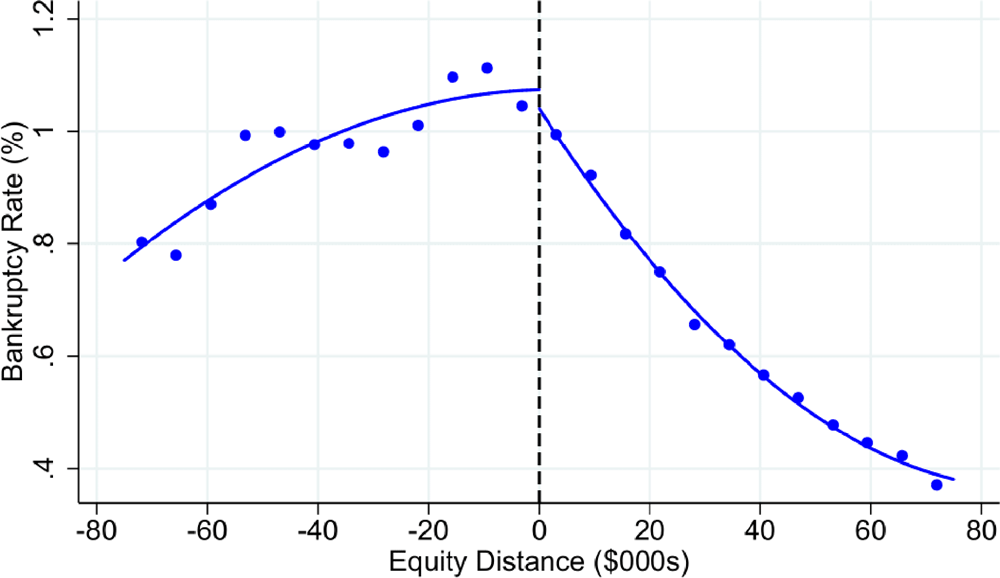
\includegraphics[width=0.9\textwidth,height=0.78\textheight,keepaspectratio]{images/figure_2_seizable_equity.png}
        \par\smallskip
    \end{center}
    {\tiny Source: Indarte (2023), Figure 2.}
\end{frame}

\begin{frame}{RKD Robustness}

    \begin{alertblock}{Identification Assumption:}
        The density of unobserved factors that affect bankruptcy decision is smooth at kink
    \end{alertblock}
    
    \vspace{0.3cm}

    \textbf{Robustness Tests:}

    \begin{itemize}
        \item Underwriting variables available at origination smoothly affects bankruptcy around kink
        \item Manipulation of home equity before bankruptcy?
        \begin{itemize}
            \item Equity distance distribution smooth at kink
        \end{itemize} 
        \item Likelihood of bankruptcy costs higher if non-exempt equity? 
        \begin{itemize}
            \item Equity distance has smooth effect on future house sales
        \end{itemize}
        \item Kinked credit supply?
        \begin{itemize}
            \item Uses household-level debt data and finds no kink
        \end{itemize}
    \end{itemize}

\end{frame}

\begin{frame}{RKD Measurement Error}
\small

\begin{alertblock}{Challenge:}
   House prices not observed creating measurement error
\end{alertblock}

Takes parametric approach to correct measurement error:
\begin{itemize}
    \item assumes outcome is quadratic in running and policy variables
    \item assumes classical measurement error in running variable
\end{itemize}

This gives the following measurement error adjustment:
\[
    \lambda =
    \left[
        \underbrace{\left(1-\frac{\widehat{\sigma}_{\mu}^{2}}{\widehat{\sigma}_{x}^{2}}\right)}_{\text{attenuation bias}}
        \underbrace{\left(1-\widehat{\pi}^{+}-\widehat{\pi}^{-}\right)}_{\text{assignment bias}}
    \right]^{-1}
    \approx 1.61.
\]
{\footnotesize
\begin{itemize}
    \item $\sigma_{\mu}^{2}/\sigma_x^{2}=0.22$: classical attenuation bias
    \item $\pi^{+}=0.109$ ($\pi^{-}=0.095$): probability observed value is on wrong side of kink
\end{itemize}
}

Perhaps with AI you could find home values from bankruptcy proceedings

\end{frame}

\begin{frame}{Results: Moral Hazard Effect}
    \centering
    % Include with % Include with % Include with \input{images/rkd_table.tex}.
\begin{minipage}{\textwidth}
\centering
\textbf{The Effect of Bankruptcy Costs on Filing (RKD Estimates)}
\par\medskip
{\small
\setlength{\tabcolsep}{7pt}
\begin{tabular}{lcccc}
\hline
\hline
 & (1) & (2) & (3) & (4) \\ \\
\hline
RK Estimate (percent of average) & $-1.64^{***}$ & $-2.63^{***}$ & $-2.31^{***}$ & $-2.36^{***}$ \\
Standard Error & (0.21) & (0.34) & (0.43) & (0.45) \\[0.2cm]
\hline
Bandwidth & 67.06 & 67.06 & 49.42 & 89.30 \\
Measurement error correction & & $\checkmark$ & $\checkmark$ & $\checkmark$ \\
RKD polynomial order & 2 & 2 & 2 & 3 \\
Home equity control order & 1 & 1 & 3 & 3 \\
\hline
LHS effective observations & 21,383,503 & 21,383,503 & 17,536,206 & 25,884,133 \\
RHS effective observations & 24,637,614 & 24,637,614 & 20,013,724 & 29,029,069 \\
\hline
Total observations & \multicolumn{4}{c}{99,233,172} \\
\hline
\hline
\end{tabular}
}
\par\medskip
\end{minipage}
.
\begin{minipage}{\textwidth}
\centering
\textbf{The Effect of Bankruptcy Costs on Filing (RKD Estimates)}
\par\medskip
{\small
\setlength{\tabcolsep}{7pt}
\begin{tabular}{lcccc}
\hline
\hline
 & (1) & (2) & (3) & (4) \\ \\
\hline
RK Estimate (percent of average) & $-1.64^{***}$ & $-2.63^{***}$ & $-2.31^{***}$ & $-2.36^{***}$ \\
Standard Error & (0.21) & (0.34) & (0.43) & (0.45) \\[0.2cm]
\hline
Bandwidth & 67.06 & 67.06 & 49.42 & 89.30 \\
Measurement error correction & & $\checkmark$ & $\checkmark$ & $\checkmark$ \\
RKD polynomial order & 2 & 2 & 2 & 3 \\
Home equity control order & 1 & 1 & 3 & 3 \\
\hline
LHS effective observations & 21,383,503 & 21,383,503 & 17,536,206 & 25,884,133 \\
RHS effective observations & 24,637,614 & 24,637,614 & 20,013,724 & 29,029,069 \\
\hline
Total observations & \multicolumn{4}{c}{99,233,172} \\
\hline
\hline
\end{tabular}
}
\par\medskip
\end{minipage}
.
\begin{minipage}{\textwidth}
\centering
\textbf{The Effect of Bankruptcy Costs on Filing (RKD Estimates)}
\par\medskip
{\small
\setlength{\tabcolsep}{7pt}
\begin{tabular}{lcccc}
\hline
\hline
 & (1) & (2) & (3) & (4) \\ \\
\hline
RK Estimate (percent of average) & $-1.64^{***}$ & $-2.63^{***}$ & $-2.31^{***}$ & $-2.36^{***}$ \\
Standard Error & (0.21) & (0.34) & (0.43) & (0.45) \\[0.2cm]
\hline
Bandwidth & 67.06 & 67.06 & 49.42 & 89.30 \\
Measurement error correction & & $\checkmark$ & $\checkmark$ & $\checkmark$ \\
RKD polynomial order & 2 & 2 & 2 & 3 \\
Home equity control order & 1 & 1 & 3 & 3 \\
\hline
LHS effective observations & 21,383,503 & 21,383,503 & 17,536,206 & 25,884,133 \\
RHS effective observations & 24,637,614 & 24,637,614 & 20,013,724 & 29,029,069 \\
\hline
Total observations & \multicolumn{4}{c}{99,233,172} \\
\hline
\hline
\end{tabular}
}
\par\medskip
\end{minipage}

\end{frame}


\begin{frame}[plain]
    \centering
    {\usebeamercolor[fg]{frametitle}\Huge\bfseries Liquidity Effect}
\end{frame}

\begin{frame}{Differential Index Rates}
    \centering
    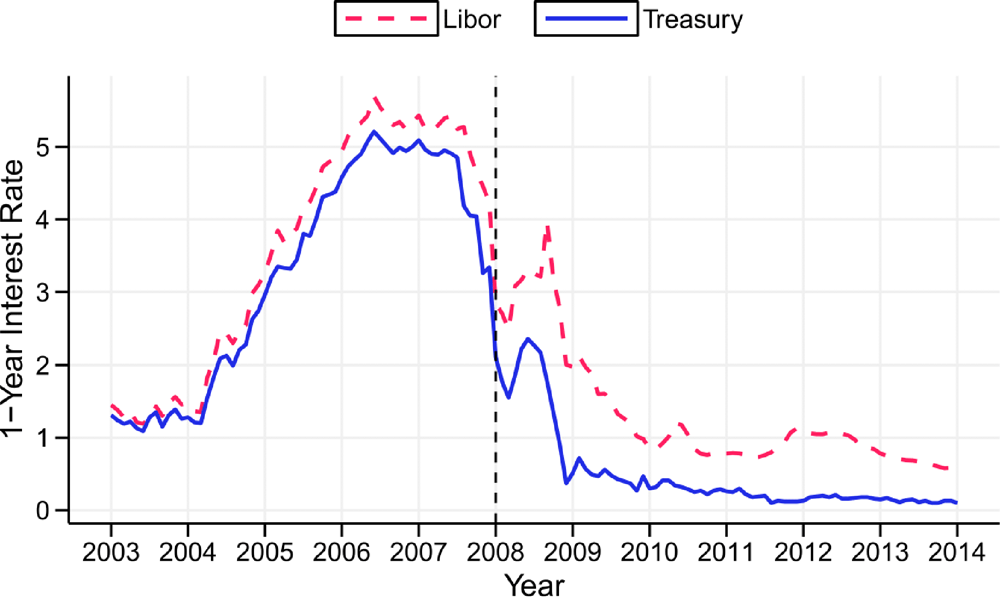
\includegraphics[width=0.9\textwidth,height=0.78\textheight,keepaspectratio]{images/figure_3_libor_treasury.png}
    \par\smallskip
    {\tiny Source: Indarte (2023), Figure 3. Monthly one-year Libor and Treasury rates.}
\end{frame}

\begin{frame}{Results: Liquidity Effect}
    \centering
    % Include with % Include with % Include with \input{images/liquidity_iv_table.tex}.
\begin{minipage}{\textwidth}
\centering
\textbf{IV Estimates of Filing Response to Liquidity}
\par{\small NPV and Composition Adjusted}
\par\smallskip
{\scriptsize
\setlength{\tabcolsep}{9pt}
\renewcommand{\arraystretch}{1.08}
\begin{tabular*}{\textwidth}{@{\extracolsep{\fill}}lcccc@{}}
\hline
\hline
 & (1) & (2) & (3) & (4) \\
\hline
\multicolumn{5}{c}{\rule{0pt}{2.6ex}\textbf{Panel A: Second stage} (Dependent Variable: Bankruptcy)} \\[0.08cm]
\hline
Mortgage Payment & $11.81^{***}$ & $11.01^{***}$ & $14.83^{***}$ & $12.59^{***}$ \\
 & (2.96) & (3.22) & (3.37) & (3.47) \\[0.1cm]
\hline
\multicolumn{5}{c}{\rule{0pt}{2.6ex}\textbf{Panel B: First stage} (Dependent Variable: Mortgage Payment)} \\[0.08cm]
\hline
Index Rate & $4{,}866.52^{***}$ & $4{,}671.64^{***}$ & $5{,}136.90^{***}$ & $5{,}179.40^{***}$ \\
 & (287.82) & (312.31) & (361.54) & (367.44) \\
\hline
Stage 1 F-Statistic & 285.89 & 223.76 & 201.88 & 198.69 \\
Observations & 1,059,194 & 1,059,194 & 1,059,194 & 1,059,194 \\
\hline
Time FE & $\checkmark$ & $\checkmark$ & $\checkmark$ & $\checkmark$ \\
County FE & $\checkmark$ & $\checkmark$ & $\checkmark$ & $\checkmark$ \\
Loan Age FE & & $\checkmark$ & $\checkmark$ & $\checkmark$ \\
Loan Age $\times$ Time FE & & & $\checkmark$ & $\checkmark$ \\
County $\times$ Time FE & & & & $\checkmark$ \\
\hline
\hline
\end{tabular*}
}
\par\smallskip
{\tiny\raggedright
Source: Indarte (2023), Table III. NPV and DFL composition adjustments applied; standard errors clustered by county. First-stage coefficients measure dollar changes in the NPV of mortgage payments per percentage-point change in the index rate.
Controls: ARM margin, original payment, origination FICO and LTV, log mortgage balance, and log home equity.
\par}
\end{minipage}
.
\begin{minipage}{\textwidth}
\centering
\textbf{IV Estimates of Filing Response to Liquidity}
\par{\small NPV and Composition Adjusted}
\par\smallskip
{\scriptsize
\setlength{\tabcolsep}{9pt}
\renewcommand{\arraystretch}{1.08}
\begin{tabular*}{\textwidth}{@{\extracolsep{\fill}}lcccc@{}}
\hline
\hline
 & (1) & (2) & (3) & (4) \\
\hline
\multicolumn{5}{c}{\rule{0pt}{2.6ex}\textbf{Panel A: Second stage} (Dependent Variable: Bankruptcy)} \\[0.08cm]
\hline
Mortgage Payment & $11.81^{***}$ & $11.01^{***}$ & $14.83^{***}$ & $12.59^{***}$ \\
 & (2.96) & (3.22) & (3.37) & (3.47) \\[0.1cm]
\hline
\multicolumn{5}{c}{\rule{0pt}{2.6ex}\textbf{Panel B: First stage} (Dependent Variable: Mortgage Payment)} \\[0.08cm]
\hline
Index Rate & $4{,}866.52^{***}$ & $4{,}671.64^{***}$ & $5{,}136.90^{***}$ & $5{,}179.40^{***}$ \\
 & (287.82) & (312.31) & (361.54) & (367.44) \\
\hline
Stage 1 F-Statistic & 285.89 & 223.76 & 201.88 & 198.69 \\
Observations & 1,059,194 & 1,059,194 & 1,059,194 & 1,059,194 \\
\hline
Time FE & $\checkmark$ & $\checkmark$ & $\checkmark$ & $\checkmark$ \\
County FE & $\checkmark$ & $\checkmark$ & $\checkmark$ & $\checkmark$ \\
Loan Age FE & & $\checkmark$ & $\checkmark$ & $\checkmark$ \\
Loan Age $\times$ Time FE & & & $\checkmark$ & $\checkmark$ \\
County $\times$ Time FE & & & & $\checkmark$ \\
\hline
\hline
\end{tabular*}
}
\par\smallskip
{\tiny\raggedright
Source: Indarte (2023), Table III. NPV and DFL composition adjustments applied; standard errors clustered by county. First-stage coefficients measure dollar changes in the NPV of mortgage payments per percentage-point change in the index rate.
Controls: ARM margin, original payment, origination FICO and LTV, log mortgage balance, and log home equity.
\par}
\end{minipage}
.
\begin{minipage}{\textwidth}
\centering
\textbf{IV Estimates of Filing Response to Liquidity}
\par{\small NPV and Composition Adjusted}
\par\smallskip
{\scriptsize
\setlength{\tabcolsep}{9pt}
\renewcommand{\arraystretch}{1.08}
\begin{tabular*}{\textwidth}{@{\extracolsep{\fill}}lcccc@{}}
\hline
\hline
 & (1) & (2) & (3) & (4) \\
\hline
\multicolumn{5}{c}{\rule{0pt}{2.6ex}\textbf{Panel A: Second stage} (Dependent Variable: Bankruptcy)} \\[0.08cm]
\hline
Mortgage Payment & $11.81^{***}$ & $11.01^{***}$ & $14.83^{***}$ & $12.59^{***}$ \\
 & (2.96) & (3.22) & (3.37) & (3.47) \\[0.1cm]
\hline
\multicolumn{5}{c}{\rule{0pt}{2.6ex}\textbf{Panel B: First stage} (Dependent Variable: Mortgage Payment)} \\[0.08cm]
\hline
Index Rate & $4{,}866.52^{***}$ & $4{,}671.64^{***}$ & $5{,}136.90^{***}$ & $5{,}179.40^{***}$ \\
 & (287.82) & (312.31) & (361.54) & (367.44) \\
\hline
Stage 1 F-Statistic & 285.89 & 223.76 & 201.88 & 198.69 \\
Observations & 1,059,194 & 1,059,194 & 1,059,194 & 1,059,194 \\
\hline
Time FE & $\checkmark$ & $\checkmark$ & $\checkmark$ & $\checkmark$ \\
County FE & $\checkmark$ & $\checkmark$ & $\checkmark$ & $\checkmark$ \\
Loan Age FE & & $\checkmark$ & $\checkmark$ & $\checkmark$ \\
Loan Age $\times$ Time FE & & & $\checkmark$ & $\checkmark$ \\
County $\times$ Time FE & & & & $\checkmark$ \\
\hline
\hline
\end{tabular*}
}
\par\smallskip
{\tiny\raggedright
Source: Indarte (2023), Table III. NPV and DFL composition adjustments applied; standard errors clustered by county. First-stage coefficients measure dollar changes in the NPV of mortgage payments per percentage-point change in the index rate.
Controls: ARM margin, original payment, origination FICO and LTV, log mortgage balance, and log home equity.
\par}
\end{minipage}

\end{frame}

\begin{frame}{Comment: Uncertain Home Values}
    \input{images/attenuation_numbers.tex}
    Homeowner's uncertainty about home value attenuates moral hazard effect
    \begin{itemize}
        \item With uncertainty, moral hazard effect \textbf{\UncertaintyMultiplier{}} times larger.
        \item Also with risk aversion, moral hazard effect \textbf{\RiskAversionMultiplier{}} times larger
    \end{itemize}
    \textcolor{blue}{$\rightarrow$} After adjustment, moral hazard effect is as large as liquidity effect

    \begin{center}
        \includegraphics[width=0.95\textwidth,height=0.52\textheight,keepaspectratio]{images/attenuation.png}
        \par\smallskip
    \end{center}
    {\tiny Asumptions: standard devation in home price uncertainty of \$\MeasurementErrorSD{} (conservative estimate if household is as uncertain as econometrician); bankruptcy wealth of \$\BaselineWealth{}; CRRA risk-aversion coefficient of \RiskAversionCoefficient{}.}
\end{frame}

\begin{frame}{Comment: Debt Forgiveness on Stressed Borrowers}
    \begin{alertblock}{Punchline:}
        If you decrease dischargeable debt, \textbf{83\%} of filing response is due to \textbf{liquidity}
    \end{alertblock}

    \vspace{0.3cm}

    To convert empirical results into terms of dischargeable debt paper assumes:
    \begin{alertblock}{Assumption 1:}
        One dollar reduction in bankruptcy generosity is equivalent to one dollar decrease in dischargeable debt
    \end{alertblock}
    
    \begingroup
    \setbeamercolor{frametitle}{fg=red}
    \begin{alertblock}{Assumption 2:}
        One dollar reduction in cash-on-hand is equivalent to one dollar decrease in dischargeable debt
    \end{alertblock}
    \endgroup

    
    \begingroup
    \setbeamercolor{frametitle}{fg=red}
    \begin{alertblock}{Critique}
        The point of debt fogiveness is that lender should not expect to recoup debt anyway, making it particuarly effective during crises
    \end{alertblock}
    \endgroup
    
    \textcolor{blue}{$\rightarrow$} Say lender thinks borrower has 50\% probability of paying back, then discharging \$1K debt only costs \$500, so liquidity effect should be halved
    
\end{frame}

% \begin{frame}{Comment: Debt Forgiveness on Stressed Borrowers}

% Debt forgiveness (out of bankruptcy) is beneficial because lender does not expect to get paid back anyway

% \vspace{0.3cm}

% \begin{itemize}
%     \item Reinterpret decrease in generosity of bankruptcy as lowering principal on outstanding debt
%     \item If borrower is about to default, then face value of debt is far below par
%     \item Forgiving \$1K in principal may cost far less than giving out a \$1K stimulus check
%     \item Comparison between moral hazard and liquidity effect ignores this
%     \item Assumes borrower behaves as if they will pay back debt
% \end{itemize}

% \vspace{0.3cm}

% \textcolor{blue}{$\rightarrow$} Debt fogiveness may be more efficient at reducing filing particularly in crises

% \end{frame}

\begin{frame}
    \centering
    \vfill
    {\usebeamercolor[fg]{frametitle}\Huge\bfseries Appendix}
    \vfill
\end{frame}

\begin{frame}{References}
    \footnotesize
    \begin{thebibliography}{9}
        \bibitem[Chatterjee et~al.(2007)]{chatterjee2007}
        % Wiley citation details, standardized to author--year format.
        % https://onlinelibrary.wiley.com/doi/10.1111/j.1468-0262.2007.00806.x
        Chatterjee, S., Corbae, D., Nakajima, M., and R\'{i}os-Rull, J.-V. (2007).
        ``A Quantitative Theory of Unsecured Consumer Credit with Risk of Default.''
        \textit{Econometrica}, 75(6), 1525--1589.
        \url{https://doi.org/10.1111/j.1468-0262.2007.00806.x}

        \bibitem[Geanakoplos(2010)]{geanakoplos2010}
        % NBER and University of Chicago Press citation details, standardized to author--year format.
        % https://www.nber.org/books-and-chapters/nber-macroeconomics-annual-2009-volume-24/leverage-cycle
        Geanakoplos, J. (2010).
        ``The Leverage Cycle.''
        \textit{NBER Macroeconomics Annual}, 24(1), 1--66.
        \url{https://doi.org/10.1086/648285}

        \bibitem[Indarte(2023)]{indarte2023}
        % Wiley citation details, standardized to author--year format.
        % https://onlinelibrary.wiley.com/doi/10.1111/jofi.13263
        Indarte, S. (2023).
        ``Moral Hazard versus Liquidity in Household Bankruptcy.''
        \textit{The Journal of Finance}, 78(5), 2421--2464.
        \url{https://doi.org/10.1111/jofi.13263}
    \end{thebibliography}
\end{frame}

\end{document}
